\documentclass{beamer}
%% fink install texlive
\usetheme{Warsaw}

\usepackage{amsmath,amssymb}
\usepackage{stmaryrd}
\usepackage{graphicx}
%\usepackage{haskell}
\usepackage{code}
%\usepackage{proof}
\usepackage{theorem}
\usepackage{pstricks} 
\usepackage{listings}
\usepackage{pgf-pie} % from https://code.google.com/p/pgf-pie/



% Martin's macros
   

% groups

%%\newtheorem{lemma}{Lemma}
%%\newtheorem{definition}{Definition}
%%\newtheorem{theorem}{Theorem}
%%\newtheorem{corollary}{Corollary}
%%\newtheorem{remark}{Remark}
%%\newtheorem{conjecture}{Conjecture}
%%\newtheorem{example}{Example}

% arrays

\newcommand{\bi}{\begin{array}[t]{@{}l@{}}}
\newcommand{\ei}{\end{array}}
\newcommand{\ba}{\begin{array}}
\newcommand{\ea}{\end{array}}
\newcommand{\bda}{\[\ba}
\newcommand{\eda}{\ea\]}
\newcommand{\bp}{\begin{quote}\tt\begin{tabbing}}
\newcommand{\ep}{\end{tabbing}\end{quote}}
\newcommand{\set}[1]{\left\{
    \begin{array}{l}#1
    \end{array}
  \right\}}
\newcommand{\sset}[2]{\left\{~#1 \left|
      \begin{array}{l}#2\end{array}
    \right.     \right\}}


% symbols

\newcommand{\good}{good}
 
\newcommand{\err}{{\bf W}}
\newcommand{\VV}{{\cal V}} 
\newcommand{\GT}{{\cal T}_G}
\newcommand{\KK}{{\cal K}}
\newcommand{\TT}{{\cal T}}
\newcommand{\TC}{\mbox{\it TC}}
\newcommand{\UL}{\mbox{UL}}
\newcommand{\sUL}{\mbox{\scriptsize UL}}
\newcommand{\true}{\mbox{\sf true}}
\newcommand{\Int}{\mbox{\it Int}}
\newcommand{\Bool}{\mbox{\it Bool}}
\newcommand{\SF}{\mbox{$\cal S$}}
\newcommand{\tauvec}{\bar{\tau}}
\newcommand{\tvec}{\bar{t}}
\newcommand{\kvec}{\bar{k}}
\newcommand{\xvec}{\bar{x}}
\newcommand{\muvec}{\bar{\mu}}
\newcommand{\alphavec}{\bar{\alpha}}
\newcommand{\betavec}{\bar{\beta}}
\newcommand{\gammavec}{\bar{\gamma}}
\newcommand{\thetavec}{\bar{\theta}}
\newcommand{\deltavec}{\bar{\delta}}
\newcommand{\bvec}{\bar{b}}
\newcommand{\typo}{\Gamma}
\newcommand{\tenv}{\Gamma}
\newcommand{\typoinit}{\typo_0}
\newcommand{\static}{S}
\newcommand{\dynamic}{D}
\newcommand{\sstatic}{{\scriptstyle S}}
\newcommand{\sdynamic}{{\scriptstyle D}}
\newcommand{\BTA}{\mbox{BTA}}
\newcommand{\baseshape}{\bot}
\newcommand{\TCT}{P}
\newcommand{\Haskell}{H98}
\newcommand{\TCTinit}{P_o}

% figures, rules


\newcommand{\tlabel}[1]{\mbox{(#1)}}
\newcommand{\fig}[3]
        {\begin{figure*}[t]#3\
        \caption{\label{#1}#2}\ \hrulefill\ \end{figure*}}
\newcommand{\figurebox}[1]
        {\fbox{\begin{minipage}{\textwidth} #1 \end{minipage}}}
\newcommand{\boxfig}[3]
        {\begin{figure*}\figurebox{#3\caption{\label{#1}#2}}\end{figure*}}
\newcommand{\myirule}[2]{{\renewcommand{\arraystretch}{1.2}\ba{c} #1
                      \\ \hline #2 \ea}}

% relations, operators

\newcommand{\sat}{\mbox{\it sat}}
\newcommand{\entail}{\mbox{\it entail}}
\newcommand{\unambig}{\mbox{\it unambig}}
\newcommand{\complete}{\mbox{\it complete}}

\newcommand{\projexclusion}[1]{\mbox{$\bar{\exists}#1$}}
\newcommand{\funinst}{\mbox{\it inst}}
%%\renewcommand{\inst}{\, \vdash^{\scriptstyle i} \,}
%%\newcommand{\inst}{\, \vdash \,}
\newcommand{\ileq}{\preceq}
\newcommand{\ieq}{\simeq}
\newcommand{\topannot}[1]{|#1|}
\newcommand{\gendelta}{\mbox{\it gen}_{\delta}}
\newcommand{\genbeta}{\mbox{\it gen}_{\beta}}
\newcommand{\gen}{\mbox{\it gen}}
\newcommand{\normalize}{\mbox{\it normalize}}
\newcommand{\fail}{\mbox{\it fail}}
\newcommand{\fixpt}{\mbox{${\cal F}$}}
\newcommand{\testpa}{\mbox{${\cal T}$}}
\newcommand{\addpa}{\mbox{${\cal A}$}}
\newcommand{\matchpa}{\mbox{${\cal M}$}}
\newcommand{\refmatchpa}{\mbox{${\cal R}$}}
\newcommand{\wft}[1]{\mbox{\it wft}(#1)}
\newcommand{\tv}{\mbox{\it fv}}
\newcommand{\stv}{\mbox{\it semfv}}
\newcommand{\range}{\mbox{\it range}}
\newcommand{\lub}{\wedge}
\newcommand{\tyrel}[2]{(#1 \preceq #2)}
\newcommand{\eqty}[2]{#1=#2}
%%\newcommand{\ts}{\, \vdash \,}
\newcommand{\turns}{\, \vdash \,}
\newcommand{\tsinst}{\, \vdash^i \,}
\newcommand{\tsttv}{\, \vdash^{ttv} \,}
\newcommand{\tsUL}{\, \vdash_{\mbox{\scriptsize UL}} \,}
\newcommand{\trc}{\, \vdash_{\scriptstyle \id{inf}} \,}
\newcommand{\trcp}{\, \vdash_{\scriptstyle inf}' \,}
\newcommand{\genrel}{\, \vdash^{\scriptstyle gen} \,}
\newcommand{\asubty}[2]{(#1 \leq_a #2)}
\newcommand{\ssubty}[2]{(#1 \leq_s #2)}
\newcommand{\fsubty}[2]{(#1 \leq_f #2)}
\newcommand{\subty}[2]{(#1 \leq #2)}
\newcommand{\doubleb}[1]{[\![ #1 ]\!]}
\newcommand{\id}[1]{\mbox{\it #1}}


\newcommand{\mynote}[1]{$\spadesuit${\bf #1}$\clubsuit$}

% spacing

\newcommand{\sgap}{\quad}
\newcommand{\bgap}{\quad\quad}

% reserved words

\newcommand{\mathem}{\sf}
\newcommand{\IN}{\mbox{\mathem in}}
\newcommand{\LET}{\mbox{\mathem let}}
\newcommand{\MLET}{\mbox{\mathem mlet}}
\newcommand{\LETREC}{\mbox{\mathem letrec}}
\newcommand{\FIX}{\mbox{\mathem fix}}
\newcommand{\CASE}{\mbox{\mathem case}}
\newcommand{\TYCASE}{\mbox{\mathem typecase}}
\newcommand{\ELSE}{\mbox{\mathem else}}
\newcommand{\IF}{\mbox{\mathem if}}
\newcommand{\OF}{\mbox{\mathem of}}
\newcommand{\THEN}{\mbox{\mathem then}}
\newcommand{\INST}{\mbox{\mathem instance}}
\newcommand{\OVER}{\mbox{\mathem overload}}
\newcommand{\CLASS}{\mbox{\mathem class}}
\newcommand{\WHERE}{\mbox{\mathem where}}


%%% Local Variables: 
%%% mode: latex
%%% TeX-master: "bta"
%%% End: 


\newcommand{\beb}{\begin{exampleblock}}
\newcommand{\eeb}{\end{exampleblock}}


\newcommand{\rev}[1]{{#1}^{\mbox{\scriptsize r}}}
\newcommand{\lquo}{\backslash}
\newcommand{\rquo}{/}
\newcommand{\diff}{-}
\newcommand{\isect}{\cap}
\newcommand{\mymid}{~\redtxt{\mid}~}

\newcommand{\ignore}[1]{}

\newcommand{\magtxt}[1]{{\magenta #1}}
\newcommand{\redtxt}[1]{{\red #1}}
\newcommand{\bluetxt}[1]{{\blue #1}}
\newcommand{\greytxt}[1]{{\gray #1}}
\newcommand{\mmleq}{\leq}
\newcommand{\pow}{\^{}}
\newcommand{\venv}{\Delta}
\newcommand{\mleq}{\mbox{\tt leq}}
\newcommand{\mas}{\mbox{\tt as}}
\newcommand{\subt}{<\!:}

\newcommand{\Nturns}{\, \vdash_{\mbox{\tiny lnf}} \,}

\newenvironment{ttprog}{\begin{trivlist}\item \tt
        \begin{tabbing}}{\end{tabbing}\end{trivlist}}


\newenvironment{grammar}{%
         \begin{center} \small%
         $\begin{array}{rcll}
         }{%
         \end{array}$\end{center}\ignorespaces%
         }

\newcommand{\rem}[1]{}

\begin{document}
\lstset{language=python}

\title{ Introduction to Spark} 
\author{ \white 
 Copyright \copyright~ 2015. All Rights Reserved
Kenny Zhuo Ming Lu 
}
\institute{
\normalsize 
Kenny Lu \\ 
School of Information Technology \\ Nanyang Polytechnic
}
\date{\today} 


%\bibliographystyle{plainnat}

\frame{\titlepage} 

%\frame{\frametitle{Table of contents}\tableofcontents} 

%-------------------------------------------------------------------
%-------------------------------------------------------------------
\begin{frame}[fragile]
\frametitle{Learning Outcomes}

\begin{itemize}
 \item Discuss and identify the differences between Parallel Programming and Concurrent Programming during system design and analysis
 \item Discuss and Identify the differences between data parallelism
   and task parallelism during system design and analysis.
 \item Understand and conceptualize data paralellism using MapReduce
 \item Comprehend and develop script in Spark for data transformation
  
\end{itemize}
\end{frame}

%-------------------------------------------------------------------
%-------------------------------------------------------------------
\begin{frame}[fragile]
\frametitle{What is a parallel program?}

\beb{What is a parallel program?}
A parallel program is one that uses a {\em \redtxt{multiplicity of computational
hardware}} (e.g., several processor cores or several server nodes) to
{\em \redtxt{ perform a computation
more quickly}}. 
The aim is to arrive at the answer earlier, by
delegating different parts of the computation to different processors
that execute at the same time.
\eeb
\end{frame}


%-------------------------------------------------------------------
%-------------------------------------------------------------------
\begin{frame}[fragile]
\frametitle{Parallelism vs Concurrency}

People often compare and confuse parallelism with concurrency.
\beb{What is a concurrent program?}
By contrast, concurrency is {\em a \redtxt{program-structuring technique}} in which
there are multiple threads of control. Conceptually, the threads of
control execute "at the same time"; that is, the user sees {\em
  \redtxt{their effects interleaved}}. Whether they actually execute at the same 
time or not is an implementation detail; a concurrent program 
can execute on a single processor through interleaved execution or 
on multiple physical processors.
\eeb
\end{frame}



%-------------------------------------------------------------------
%-------------------------------------------------------------------
\begin{frame}[fragile]
\frametitle{Parallelism vs Concurrency}

\begin{tabular}{|c|c|c|}
\hline
   & Parallelism & Concurrency \\ \hline \hline
Area of Focus & Efficiency & Structural and Modularity \\ \hline
Number of Goals & One & One or more \\ \hline
Program Semantic & Deterministic & Non-deterministic \\ \hline
Single processor Exec & Sequential & Interleaving   \\ \hline \hline

\end{tabular}

\end{frame}


%-------------------------------------------------------------------
%-------------------------------------------------------------------
\begin{frame}[fragile]
\frametitle{Parallelism vs Concurrency}

Examples of Parallelism 
\begin{itemize} 
 \item A sodoku solver uses multiple CPU cores
 \item A parallelized database query that retrieves and aggregates records from a
   cluster of replica of database.
 \item A K-means analyses running over a Hadoop cluster
\end{itemize}

Examples of Concurrency
\begin{itemize}
 \item A web application that handles multiple clients HTTP requests
   and interacting with the databases.
 \item A User Interface of the a mobile phone handles user's touch screen input
   and exchanging data via the 4G network
\end{itemize}

\end{frame}


%-------------------------------------------------------------------
%-------------------------------------------------------------------

\begin{frame}[fragile]
\frametitle{Different Types of Hardware Parallelism}

\begin{itemize}
\item Single processor, e.g. 
\begin{itemize}
 \item Bit-level parallelism
 \item Instruction Pipelining
\end{itemize}
\item GPU, e.g. 
   \begin{itemize}
      \item Matrix operations parallelisation
   \end{itemize}
\item Multiple processors in a single machine
 \begin{itemize}
 \item Shared Memory
    \begin{itemize}
       \item Multi-core computer executes multi-threaded
         program. Memory are shared among different threads. 
    \end{itemize}
 \item Distributed Memory
    \begin{itemize}
      \item Multi-GPU parallelisation.
    \end{itemize}
 \end{itemize}
\item Multiple hosts (machines)
   \begin{itemize}
       \item A grid computing
       \item MapReduce cluster, Hadoop
   \end{itemize}
\end{itemize}
\end{frame}




%-------------------------------------------------------------------
%-------------------------------------------------------------------
\begin{frame}[fragile]
\frametitle{Different Types of Software Parallelism}

Software Parallelism
\begin{itemize}
 \item Task parallelism (Dataflow parallelism)
 \item Data parallelism

\end{itemize}

\end{frame}

%-------------------------------------------------------------------
%-------------------------------------------------------------------
\begin{frame}[fragile]
\frametitle{Different Types of Software Parallelism}

\beb{Task parallelism}
  \begin{code}
   def cook_beef_bolognese(beef,spaghetti) = {
     val sauce = cook_sauce(beef) // task A
     val pasta = cook_pasta(spaghetti) //  task B
     mix(sauce,pasta)
   }
   \end{code}
\eeb
Note that task A and task B can be executed in parallel, e.g. 
{\tt cook\_sauce(beef)} is executed in Core 1, 
{\tt cook\_pasta(spaghetti)} is executed in Core 2.
\end{frame}


%-------------------------------------------------------------------
%-------------------------------------------------------------------
\begin{frame}[fragile]
\frametitle{Different Types of Software Parallelism}

\beb{Data parallelism}
  \begin{code}
   def factorial(n) = ... 
   def main() {
      val inputs = List( 10, 100, 200, ...) 
      val results = List()
      for ( i <- inputs ) 
      { 
          results.append(factorial(i))
      }
      results
   }
   \end{code}
\eeb

\end{frame}



%-------------------------------------------------------------------
%-------------------------------------------------------------------
\begin{frame}[fragile]
\frametitle{Different Types of Software Parallelism}

\beb{Data parallelism}
  \begin{code}
   def factorial(n) = ... 
   def main() {
      val inputs = List( 10, 100, 200, ...) 
     // task C
      val results = inputs.map( i => factorial( i ) ) 
      results
   }
   \end{code}
\eeb
Note that each task C can be executed in parallel, e.g.
{\tt factorial(10)} is executed in Core 1,
{\tt factorial(100)} is executed in Core 2,
{\tt factorial(200)} is executed in Core 3, 
...
\end{frame}


%-------------------------------------------------------------------
%-------------------------------------------------------------------
\begin{frame}[fragile]
\frametitle{Different Types of Software Parallelism}

In most of situations, data parallelism is more scalable than task parallelism.
\end{frame}


%-------------------------------------------------------------------
%-------------------------------------------------------------------
\begin{frame}[fragile]
\frametitle{MapReduce and Google}

\begin{itemize}
 \item MapReduce was first introduced and developed by the development
   in Google \cite{Dean:2008:MSD:1327452.1327492}.
 \item MapReduce is a formed of data parallelism.
 \item MapReduce is popularized by Hadoop.
\end{itemize}
\end{frame}

%-------------------------------------------------------------------
%-------------------------------------------------------------------
\begin{frame}[fragile]
\frametitle{MapReduce's Origin}

\begin{itemize}
 \item MapReduce was inspired by two combinators coming from
   Functional Programming world, i.e. {\tt map} and {\tt
     reduce} (some times {\tt reduce} is named as {\tt fold})
 \item MapReduce exploits the concept of purity fro FP world to
   achieve parallelism.
\end{itemize}
\end{frame}


%-------------------------------------------------------------------
%-------------------------------------------------------------------
\begin{frame}[fragile]
\frametitle{{\tt map}}

In FP languages, {\tt map(f,l)} takes two formal arguments, a {\em
  higher order} function {\tt f} and a list {\tt l}, and applies {\tt f} to every element
in {\tt l}. 

For instance, let {\tt incr(x)} be a function that returns the result
of adding 1 to {\tt x}. 
\beb{incr}
\begin{code}
def incr(x) = x + 1
\end{code}
\eeb
We apply it with {\tt map} as follows
\beb{{\tt map} in action}
\begin{code}
map(incr, [1,2,3,4])
\end{code}
\eeb
evaluates to 
\beb{}
\begin{code}
[incr(1),incr(2),incr(3),incr(4)]
\end{code}
\eeb
yields
\beb{}
\begin{code}
[2,3,4,5]
\end{code}
\eeb
\end{frame}



%-------------------------------------------------------------------
%-------------------------------------------------------------------
\begin{frame}[fragile]
\frametitle{{\tt map}}

Given that {\tt f} is a {\em pure} function, (i.e. it
does not modify its external state when it is executed,)
it is guaranteed that {\tt map(f,l)} can be parallelized by applying
{\tt f} to every element in {\tt l} in parallel.

 For instance, assuming we have processors \magtxt{A}, \bluetxt{B},
 \redtxt{C} and \greytxt{D}.
\beb{{\tt map} in parallelized mode}
\begin{code}
map(incr, [1,2,3,4])
\end{code}
\eeb
evaluates to 
\beb{}
\begin{ttprog}
[\magtxt{incr(1)},\bluetxt{incr(2)},\redtxt{incr(3)},\greytxt{incr(4)}]
\end{ttprog}
\eeb
yields
\beb{}
\begin{ttprog}
[\magtxt{2},\bluetxt{3},\redtxt{4},\greytxt{5}]
\end{ttprog}
\eeb
\end{frame}

%-------------------------------------------------------------------
%-------------------------------------------------------------------
\begin{frame}[fragile]
\frametitle{More on Pure function}

A full defintiion of Pure function from Wikipedia.

A function may be described as a pure function if both these statements about the function hold:

\begin{enumerate}
\item The function always evaluates the same result value given the
  same argument value(s). The function result value cannot depend on
  any hidden information or state that may change as program execution
  proceeds or between different executions of the program, nor can it
  depend on any external input from I/O devices.
\item Evaluation of the result does not cause any semantically
  observable side effect or output, such as mutation of mutable
  objects or output to I/O devices
\end{enumerate}

\end{frame}



%-------------------------------------------------------------------
%-------------------------------------------------------------------



%-------------------------------------------------------------------
%-------------------------------------------------------------------
\begin{frame}[fragile]
\frametitle{{\tt reduce}}

{\tt reduce(f,l)} takes a  function {\tt f} and a list {\tt
  l}, it aggregates the elemeents in {\tt l} with {\tt f}.


For instance, let {\tt add(x,y)} be a function that returns the result
of adding {\tt x} to {\tt y}. 
\beb{add}
\begin{code}
def add(x,y) = x + y
\end{code}
\eeb
We apply it with {\tt reduce} as follows
\beb{{\tt reduce} in action}
\begin{code}
reduce(add, [2,3,4,5])
\end{code}
\eeb
evaluates to 
\beb{}
\begin{code}
2+3+4+5
\end{code}
\eeb
yields
\beb{}
\begin{code}
14
\end{code}
\eeb


\end{frame}

%-------------------------------------------------------------------
%-------------------------------------------------------------------
\begin{frame}[fragile]
\frametitle{{\tt reduce}}

Given {\tt f} is pure and {\em associative}, ({\tt f} is associative
iff {\tt f(x,f(y,z)) == f(f(x,y),z)}), it is guaranteed that {\tt reduce(f,l)}
can be parallelized by partitioning elements in {\tt l} into segments,
aggregating each segment with {\tt f} and aggregating the segment
results into the final result.

 For instance, assuming we have processors \magtxt{A} and \bluetxt{B}.
\beb{{\tt reduce} in parallelized mode}
\begin{code}
reduce(add, [2,3,4,5])
\end{code}
\eeb
evaluates to 
\beb{}
\begin{ttprog}
\magtxt{2+3}+\bluetxt{4+5}
\end{ttprog}
\eeb
yields
\beb{}
\begin{ttprog}
\magtxt{5+9}
\end{ttprog}
\eeb
yields {\tt 14}.
\end{frame}

%-------------------------------------------------------------------
%-------------------------------------------------------------------
\begin{frame}[fragile]

\frametitle{Tweaking the partitions in {\tt reduce}}
Suppose instead of summing up all integers in the {\tt reduce} step,
we would like to sum up all the even numbers and odd numbers
separately.

 For instance, assuming we have processors \magtxt{A}, \bluetxt{B},
 \redtxt{C} and \greytxt{D}.
\beb{{\tt map} in parallelized mode with partition keys}
\begin{code}
map(incr, [1,2,3,4])
\end{code}
\eeb
evaluates to 
\beb{}
\begin{ttprog}
[\magtxt{(0,incr(1))},\bluetxt{(1,incr(2))},\redtxt{(0,incr(3))},\greytxt{(1,incr(4))}]
\end{ttprog}
\eeb
yields
\beb{}
\begin{ttprog}
[\magtxt{(0,2)},\bluetxt{(1,3)},\redtxt{(0,4)},\greytxt{(1,5)}]
\end{ttprog}
\eeb
Note that there are two possible values appearing as the first
component of the pairs. {\tt 0} indicates that
the following value is an even number and {\tt 1} denotes the
following number is an odd number.
\end{frame}


%-------------------------------------------------------------------
%-------------------------------------------------------------------
\begin{frame}[fragile]

\frametitle{Tweaking the partitions in {\tt reduce}}
Now we can split the intermediate results into two different
lists/arrays based on the partition ids (either {\tt 0} or {\tt 1}).
\beb{}
\begin{code}
(0,[2,4])
\end{code}
\eeb
and
\beb{}
\begin{code}
(1,[3,5])
\end{code}
\eeb
\end{frame}

%-------------------------------------------------------------------
%-------------------------------------------------------------------


\begin{frame}[fragile]
\frametitle{Tweaking the partitions in {\tt reduce}}
The two partitions can be processed as two independent {\tt reduce} tasks.
\beb{{\tt reduce} the even numbers in processor A}
\begin{code}
(0, reduce([2,4]))
\end{code}
\eeb
and
\beb{{\tt reduce} the odd numbers in processor B}
\begin{code}
(1, reduce([3,5]))
\end{code}
\eeb

If we need to compute the final sum, we can run {\tt reduce} over the
results from the two tasks.
\end{frame}


%-------------------------------------------------------------------
%-------------------------------------------------------------------

\begin{frame}[fragile]
\frametitle{MapReduce in Hadoop}

Two basic components in MapReduce
\begin{itemize}
\item Mapper
\item Reducer
\end{itemize}

\end{frame}



%-------------------------------------------------------------------
%-------------------------------------------------------------------



\begin{frame}[fragile]
\frametitle{MapReduce in Hadoop}

Mapper
\begin{itemize}
 \item Input: A list/array of key-value pairs. 
 \item Output: A list/array of key-value pairs.
\end{itemize}

\end{frame}

%-------------------------------------------------------------------
%-------------------------------------------------------------------



\begin{frame}[fragile]
\frametitle{MapReduce in Hadoop}

Reducer
\begin{itemize}
 \item Input: A key and a list/array of values
 \item Output: A key and a value
\end{itemize}

\end{frame}



%-------------------------------------------------------------------
%-------------------------------------------------------------------



\begin{frame}[fragile]
\frametitle{MapReduce in Hadoop}


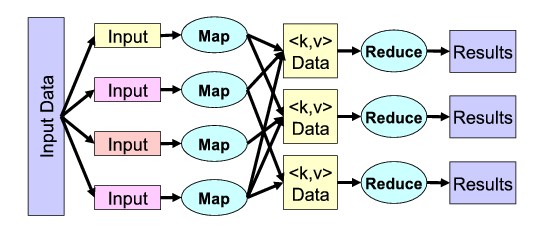
\includegraphics[height=5cm]{pic/mapreduce.png} 

\end{frame}



%-------------------------------------------------------------------
%-------------------------------------------------------------------
\begin{frame}[fragile]
\frametitle{An Example}
\beb{WordCount Not using Hadoop}
{\scriptsize
\begin{code}
val counts = new Map()
val lines = scala.io.Source.fromFile("file.txt").mkString

for (line <- lines) {
    words = line.split(" ")
    for (word <- words) {
        counts.get(word) match 
        { case None => counts.add(word,1)
          case Some(count) => counts.update(word,count + 1)
        }
    }
}
for ( (word,count) <- counts.iterator() ) {
    println(s"$word \t $count")
}\end{code}
}
\eeb
\end{frame}


%-------------------------------------------------------------------
%-------------------------------------------------------------------
\begin{frame}[fragile]
\frametitle{An Example}

Let's say the input file is as follows
\beb{}
\begin{code}
hey diddle diddle
the cat and the fiddle
the cow jumped over the 
 moon
the little dog laughed
to see such sport
and the dish ran away 
 with the spoon
\end{code}
\eeb
\end{frame}



%-------------------------------------------------------------------
%-------------------------------------------------------------------
\begin{frame}[fragile]
\frametitle{An Example}
We expect the output as 
\beb{}
{\scriptsize
\begin{code}
hey	1
diddle	2
the	7
cat	1 
and	2
fiddle	1
cow	1 
jumped	1
over	1
moon	1
little	1
dog	1
laughed	1
to	1 
see	1
such	1
sport	1
dish	1
ran	1 
away	1
with	1 
spoon	1
\end{code}
}
\eeb
\end{frame}





%-------------------------------------------------------------------
%-------------------------------------------------------------------
\begin{frame}[fragile]
\frametitle{An Example}


\beb{The Mapper for WordCount}
{\scriptsize
\begin{code}
class WordCountMapper extends Mapper[Object,Text,Text,IntWritable] {
  val one = new IntWritable(1)
  val word = new Text
  
  override
  def map(key:Object, value:Text, context:
        Mapper[Object,Text,Text,IntWritable]#Context) = {
    for (t <-  value.toString().split("\\s")) {
      word.set(t)
      context.write(word, one)
    }
  }
}
\end{code}
}
\eeb

\end{frame}

%-------------------------------------------------------------------
%-------------------------------------------------------------------
\begin{frame}[fragile]
\frametitle{An Example}


\beb{The Reducer for WordCount}
{\scriptsize
\begin{code}
class WordCountReducer extends Reducer[Text,IntWritable,Text,IntWritable] {
  override
  def reduce(key:Text, values:java.lang.Iterable[IntWritable], 
        context:Reducer[Text,IntWritable,Text,IntWritable]#Context) = {
    val sum = values.foldLeft(0) { (t,i) => t + i.get }
    context.write(key, new IntWritable(sum))
  }
}\end{code}
}
\eeb

\end{frame}


%-------------------------------------------------------------------
%-------------------------------------------------------------------
\begin{frame}[fragile]
\frametitle{An Example}


\beb{Main for WordCount}
{\scriptsize
\begin{code}
object WordCount {

  def main(args:Array[String]):Int = {
    val conf = new Configuration()
    val otherArgs = new GenericOptionsParser(conf, args).getRemainingArgs
    if (otherArgs.length != 2) {
      println("Usage: wordcount <in> <out>")
      return 2
    }
    val job = Job.getInstance(conf, "wordcount");
    job.setJarByClass(classOf[WordCountMapper])
    job.setMapperClass(classOf[WordCountMapper])
    job.setCombinerClass(classOf[WordCountReducer])
    job.setReducerClass(classOf[WordCountReducer])
    job.setOutputKeyClass(classOf[Text])
    job.setOutputValueClass(classOf[IntWritable])
    FileInputFormat.addInputPath(job, new Path(args(0)))
    FileOutputFormat.setOutputPath(job, new Path((args(1))))
    if (job.waitForCompletion(true)) 0 else 1
  }
}
// yarn jar yourJar.jar WordCount /input/ /output/
\end{code}
}
\eeb

\end{frame}

%-------------------------------------------------------------------
%-------------------------------------------------------------------
\begin{frame}[fragile]
\frametitle{An Example}

\beb{Let's say the input file is as follows}
{\scriptsize
\begin{code}
hey diddle diddle
the cat and the fiddle
the cow jumped over the 
 moon
the little dog laughed
to see such sport
and the dish ran away 
 with the spoon
\end{code}
}
\eeb
\end{frame}


%-------------------------------------------------------------------
%-------------------------------------------------------------------
\begin{frame}[fragile]
\frametitle{An Example}

\beb{The mappers go through line by line}
{\scriptsize
\begin{code}
[("hey",1), ("diddle",1), ("diddle",1)]
the cat and the fiddle
the cow jumped over the 
 moon
the little dog laughed
to see such sport
and the dish ran away 
 with the spoon
\end{code}
}
\eeb
\end{frame}

%-------------------------------------------------------------------
%-------------------------------------------------------------------
\begin{frame}[fragile]
\frametitle{An Example}

\beb{The mappers go through line by line}
{\scriptsize
\begin{code}
[("hey",1), ("diddle",1), ("diddle",1)]
[("the",1), ("cat",1), ("and",1), ("the",1), ("fiddle", 1)]
the cow jumped over the 
 moon
the little dog laughed
to see such sport
and the dish ran away with 
 the spoon
\end{code}
}
\eeb
\end{frame}
%-------------------------------------------------------------------
%-------------------------------------------------------------------
\begin{frame}[fragile]
\frametitle{An Example}

\beb{The mappers go through line by line}
{\scriptsize
\begin{code}
[("hey",1), ("diddle",1), ("diddle",1)]
[("the",1), ("cat",1), ("and",1), ("the",1), ("fiddle", 1)]
[("the",1), ("cow",1), ("jumped",1), ("over",1), ("the", 1),
 ("moon", 1)]
[("the",1), ("little",1), ("dog",1), ("laughed", 1)]
[("to",1), ("see",1), ("such",1), ("sport",1)]
[("and",1), ("the",1), ("dish",1), ("ran",1), ("away",1),
 ("with",1), ("the",1), ("spoon",1)]
\end{code}
}
\eeb
\end{frame}


%-------------------------------------------------------------------
%-------------------------------------------------------------------
\begin{frame}[fragile]
\frametitle{An Example}

\beb{The output from the mappers are grouped by keys}
{\scriptsize
\begin{code}
[("hey",[1]),
 ("diddle",[1,1]),
 ("the",[1,1,1,1,1,1,1]),
 ("cat",[1]), 
 ("and",[1,1]),
 ("fiddle", [1]),
 ("cow",[1]), 
 ("jumped",[1]), 
 ("over",[1]),
 ("moon", [1]),
 ("little",[1]), 
 ("dog",[1]), 
 ("laughed", [1]),
 ("to",[1]), 
 ("see",[1]), 
 ("such",[1]),
 ("sport",[1])
 ("dish",[1]), 
 ("ran",[1]), 
 ("away",[1]),
 ("with",[1]), 
 ("spoon",[1])]
\end{code}
}
\eeb
\end{frame}

%-------------------------------------------------------------------
%-------------------------------------------------------------------
\begin{frame}[fragile]
\frametitle{An Example}
\beb{The reducers sum up the values for each key}
{\scriptsize
\begin{code}
[("hey",1),
 ("diddle",2),
 ("the",7),
 ("cat",1), 
 ("and",2),
 ("fiddle", 1),
 ("cow",1), 
 ("jumped",1), 
 ("over",1),
 ("moon", 1),
 ("little",1), 
 ("dog",1), 
 ("laughed", 1),
 ("to",1), 
 ("see",1), 
 ("such",1),
 ("sport",1)
 ("dish",1), 
 ("ran",1), 
 ("away",1),
 ("with",1), 
 ("spoon",1)]
\end{code}
}
\eeb
\end{frame}


%-------------------------------------------------------------------
%-------------------------------------------------------------------
\begin{frame}
\frametitle{What's wrong with Hadoop?}
\begin{itemize}
\item All the mapper and reducers are communicating via the HDFS
\item Reducers tend to be the bottle neck and its loads hardly
  re-distribute!
\end{itemize}
\end{frame}






%-------------------------------------------------------------------
%-------------------------------------------------------------------
\begin{frame}
\frametitle{What is Spark?}
\begin{itemize}
\item A distrbute cluster computing system favoring in-memory computation. 
\item It was developed intially for batch processing computation like MapReduce
\end{itemize}
\end{frame}


%-------------------------------------------------------------------
%-------------------------------------------------------------------
\begin{frame}
\frametitle{Why Spark?}
What's wrong with MapReduce?
\begin{itemize}
 \item  it was designed for moderate CPU and low memory systems. 
 \item  it relies on disk I/O operations at each intermediate steps. 
 \item Its performance is capped by the disk I/O performance, and symmetric distribution of the
Reduce jobs.
\end{itemize}
Spark comes in assuming our machines are in general more powerful, and
RAMs are cheaper. 
\begin{itemize}
\item it favors in memory computations. Data are loaded from disk and
  stay in memory as long as possible.
\item it uses resillent distributed datasets (RDD) as the abstract data collections.
\item it performs better than MapReduce if we have sufficient RAM in
  the cluster.
\end{itemize}
\end{frame}



%-------------------------------------------------------------------
%-------------------------------------------------------------------
\ignore{
\begin{frame}
\frametitle{Spark vs Hadoop MapReduce}

\begin{tabular}{|c|c|c|} \hline
 & Spark & HD MR \\ \hline \hline 
Objectives & Data volume & Data volume \\ \hline 
Type of parallelism & Data & Data \\ \hline 
Task life-time  & Fixed & Fixed \\  \hline 
Input  & Block and batch data  & Block and batch data \\ \hline 
Roles & Master and workers & Master and slaves \\  \hline 
Components & Driver programs & Mappers and reducers \\ \hline 
Task  & Jobs & Jobs \\ \hline
\end{tabular}
\end{frame}
}
%-------------------------------------------------------------------
%-------------------------------------------------------------------
\begin{frame}[fragile]
\frametitle{Spark Architecture}

\begin{figure}[!htb]
\centering
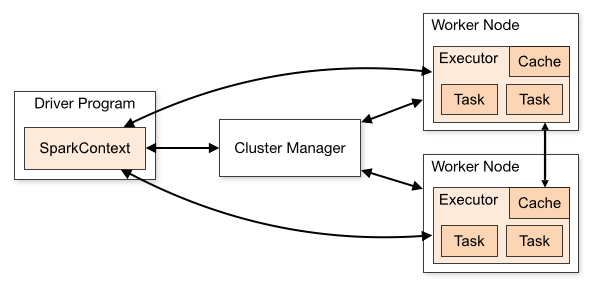
\includegraphics[scale=0.5]{pic/spark.png}
\end{figure}

A SparkContext is an interface between the Spark Driver Program
  (application) and the Spark runtime-system

\end{frame}



%-------------------------------------------------------------------
%-------------------------------------------------------------------
\begin{frame}[fragile]
\frametitle{WordCount Example in Spark}

\beb{Wordcount in Scala} 
\begin{code}
val lines = sc.textFile("hdfs://127.0.0.1:9000/input/")
val counts = lines.flatMap(line => line.split(" "))
    .map(word => (word, 1))
    .reduceByKey(_ + _)
counts.saveAsTextFile("hdfs://127.0.0.1:9000/output/")
\end{code} \eeb

\beb{Wordcount in Python}
\begin{code}
lines = sc.textFile("hdfs://127.0.0.1:9000/input/")
counts = lines.flatMap(lambda x: x.split(' ')) \
              .map(lambda x: (x, 1)) \
              .reduceByKey(add)
couts.saveAsTextFile("hdfs://127.0.0.1:9000/output/")
\end{code} \eeb
{\tt sc} denotes SparkContext 
\end{frame}




%-------------------------------------------------------------------
%-------------------------------------------------------------------
\begin{frame}[fragile]
\frametitle{WordCount Example in Spark}

\beb{Wordcount in Scala} 
\begin{code}
val lines:RDD[String] = 
    sc.textFile("hdfs://127.0.0.1:9000/input/")
val counts:RDD[(String,Long)] = 
    lines.flatMap(line => line.split(" "))
    .map(word => (word, 1))
    .reduceByKey(_ + _)
counts.saveAsTextFile("hdfs://127.0.0.1:9000/output/")
\end{code} \eeb
Recall in Scala {\tt  List(1,2,3).map( v => v + 1) }
yields  {\tt List(2,3,4) } \\ 
and {\tt List(List(1),List(2),List(3)).flatMap( l => l ) } 
yields
{\tt List(1,2,3) }
\\
An RDD can be seen as a distributed list. 
\end{frame}


%-------------------------------------------------------------------
%-------------------------------------------------------------------
\begin{frame}[fragile]
\frametitle{Resilient Distributed Dataset}

\begin{itemize} 
\item RDD is an abstraction over a collection of data set being distributed
and partitioned across a cluster of worker machines, mostly in memory.
\item Programmers are not required to manage or to coordinate that
distributed and partitioned. RDD is fault tolerant.  
\item RDDs are initialized and managed by the SparkContext.
\end{itemize}
\end{frame}




%-------------------------------------------------------------------
%-------------------------------------------------------------------


\begin{frame}[fragile]
\frametitle{RDD transformations are pure}

\begin{figure}[!htb]
\centering
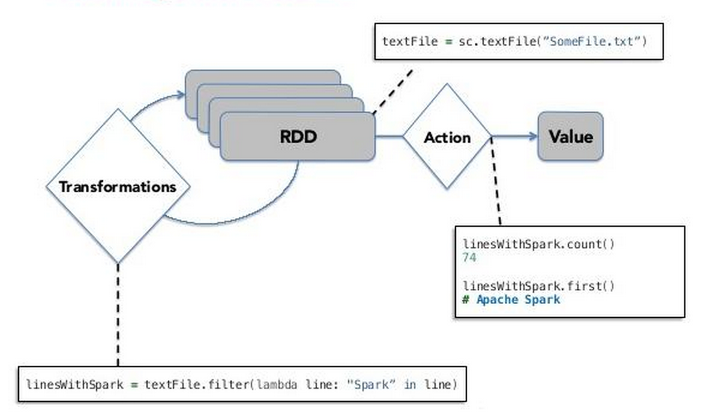
\includegraphics[scale=0.5]{pic/spark-rdd-partition-and-spark-rdd-architecture.png}
\end{figure}
Image adapted from {\tt http://www.hadooptpoint.com}

\end{frame}




%-------------------------------------------------------------------
%-------------------------------------------------------------------


\begin{frame}[fragile]
\frametitle{RDD transformations are pure}



Let {\tt r} denotes an RDD,
\begin{itemize}
\item {\tt r.map(f)} and {\tt r.flatMap(f)} applies {\tt f} to
  elements in {\tt r}.
\item {\tt r.filter(f)} filters away elements {\tt x} in {\tt r} which {\tt
    f(x)} yields {\tt false}.
\item assuming {\tt r} is a collection of key-value pairs, {\tt r.reduceByKey(f)} will
  shuffle the pairs and group them by keys. The values grouped under the same key will be
  reduced by {\tt f}. Data locality is exploit when possible.
\end{itemize}

\end{frame}



%-------------------------------------------------------------------
%-------------------------------------------------------------------


\begin{frame}[fragile]
\frametitle{RDD transformations are lazy}

\begin{itemize}
\item Computations do not take place unless the results are needed.
\item In memory cache are explicitly created.
\end{itemize}
\beb{Wordcount in Scala} 
\begin{code}
val lines:RDD[String] = 
    sc.textFile("hdfs://127.0.0.1:9000/input/")
val counts:RDD[(String,Long)] = 
    lines.flatMap(line => line.split(" "))
    .map(word => (word, 1))
    .reduceByKey(_ + _)
counts.persist() // caching
counts.saveAsTextFile("hdfs://127.0.0.1:9000/output/")
val somethingelse = counts.map( ... )
\end{code} \eeb

\end{frame}


%-------------------------------------------------------------------
%-------------------------------------------------------------------


\begin{frame}[fragile]
\frametitle{RDD transformations are resilient to node failure}

Since computations are pure, hence they are deterministic. 
Final results and intermediate results can be always recomputed.
\end{frame}





%-------------------------------------------------------------------
%-------------------------------------------------------------------



\begin{frame}[fragile]
\frametitle{How to run it?}

First start the cluster
\begin{code}
$ /opt/spark-1.4.1-bin-hadoop2.6/sbin/start-all.sh
\end{code}
%$
\end{frame}
%-------------------------------------------------------------------
%-------------------------------------------------------------------

\begin{frame}[fragile]
\frametitle{Run it in the REPL}

\beb{}
\begin{code}
$ /opt/spark-1.4.1-bin-hadoop2.6/bin/spark-shell
 scala> :load Wordcount.scala
\end{code}
%$
\eeb
Or we can type the code in line by line. 
\end{frame}


%-------------------------------------------------------------------
%-------------------------------------------------------------------

\begin{frame}[fragile]
\frametitle{Submit to the cluster}

\beb{Scala}
\begin{code}
$ /opt/spark-1.4.1-bin-hadoop2.6/bin/spark-submit
 Wordcount.jar
\end{code}
%$
\eeb

\beb{Python}
\begin{code}
$ /opt/spark-1.4.1-bin-hadoop2.6/bin/spark-submit 
wordcount.py
\end{code}
%$
\eeb

It supports R too.
\end{frame}


\end{document}
